\subsection{Описание прочих изменений в конфигурации}
\marginnote{\Date{Пт.}{30}{Июня}{2017}}[20pt]
\subsubsection{Показ остатков в кассе}
\begin{itemize}	
	\item При выборе на кассе кличества товара большего чем есть на остатках выводилось сообщение оп превышении остатка с не хватающим количеством, что позволяло косвенным образом узнать остаток товара на складе.\par
	Сообщение изменено, количество недостающего товара не показывается.
\end{itemize}	
\subsubsection{Контроль движения возвратной тары}	 
\begin{itemize}	
	\item Возвратная тара теперь может двигаться только документами "<Поступление товаров"> и "<Возврат товаров поставщику">. При наличии возвратной тары  в табличной части "<товары"> других документов, эти документы не проводятся.  
\marginnote{\Date{Чт.}{27}{Июля}{2017}}[20pt]	
	\item Добавлена константа "<крюДатаНачалаУчетаКег"> для того, что бы документы более ранней даты при перепроведении не делали движения по регистру "<Тара на складах">.  
\end{itemize}			


%	\begin{figure}[H]
%		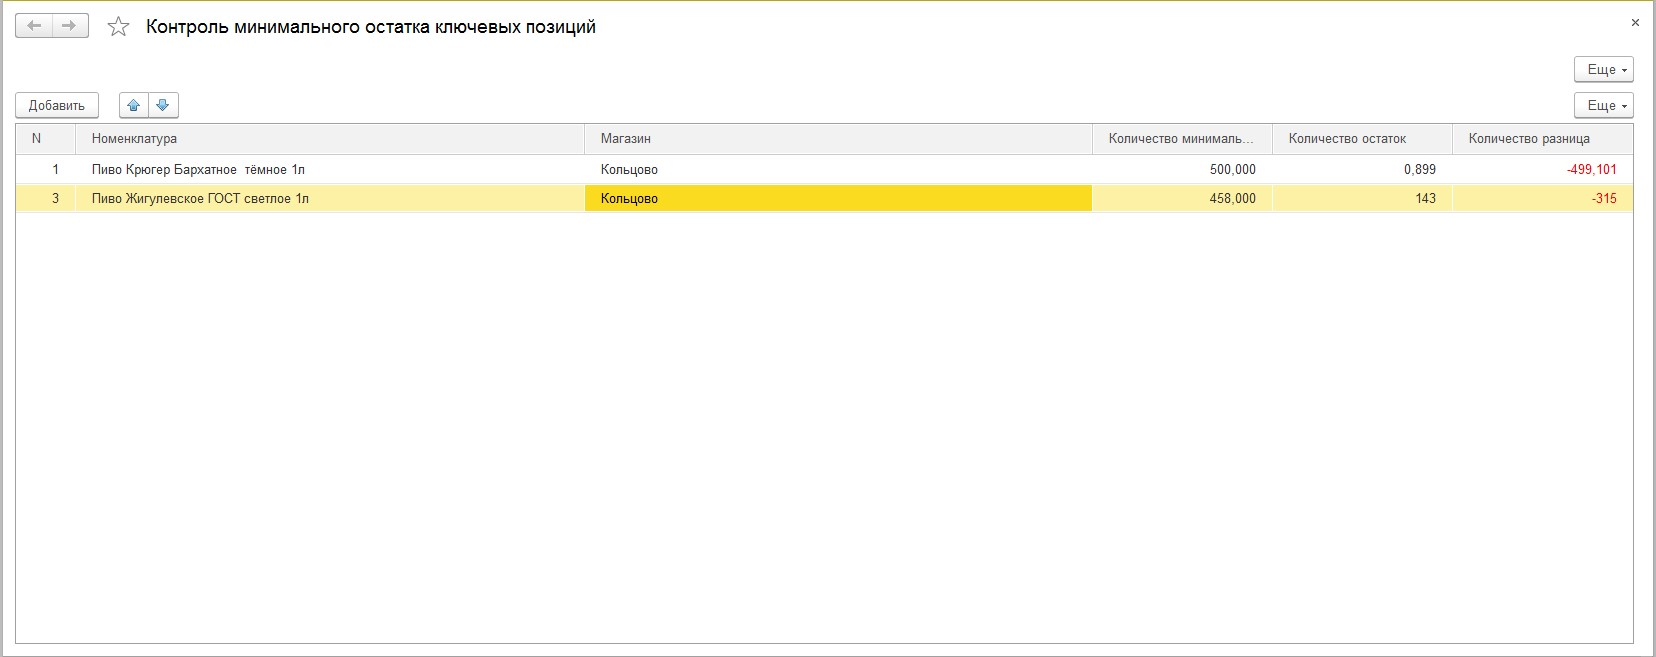
\includegraphics[width=0.90\textwidth]{10_1.jpg}
%		\caption{Старт при запуске системы.}
%		\label{ris:10_1.jpg}
%	\end{figure}

